\documentclass[spanish, c]{beamer}

\usepackage[utf8]{inputenc}
%\usepackage[spanish, mexico]{babel}
\usepackage{amsmath}
\usepackage{mathtools}
\usepackage{hyperref}
\usepackage{xcolor}
\usepackage{color}
\usepackage{ragged2e}
\usepackage{mathrsfs}
\usepackage{csquotes}
\usepackage{listings}
\usepackage[scaled]{beramono}
\usepackage[T1]{fontenc}
\usepackage{matlab-prettifier}
\usepackage{graphicx}
\usepackage{booktabs}
\usepackage{gensymb}

\renewcommand{\indent}{\hspace*{2em}}

% \usepackage{tikz}

% \usetikzlibrary{fit, shapes, arrows}

% \usepackage{courier}
% \usepackage{subfigure}
% \usepackage{enumerate}
% \usepackage{algorithmic}
% \usepackage{algorithm}

% \usepackage{listings}
% \usepackage{lstlinebgrd}

\usetheme{Boadilla}
\usefonttheme[onlymath]{serif}

\newcommand{\matlab}[1]{\lstinline[style=Matlab-editor]!#1!}
\newcommand\blfootnote[1]{%
\begingroup
\renewcommand\thefootnote{}\footnote{#1}%
\addtocounter{footnote}{-1}%
\endgroup
}

\lstset
{
    language = Matlab,
    style = Matlab-editor,
    basicstyle = \mlttfamily\scriptsize,
    escapechar = `,
    numbers = left,
    frame = tb,
}

\lstdefinestyle{output}
{
    language = {},
    basicstyle = \mlttfamily\scriptsize,
    escapechar = `,
    numbers = none,
    showtabs = false,
   	showstringspaces = false,
}

\makeatletter
\renewcommand*\env@matrix[1][*\c@MaxMatrixCols c]{%
  \hskip -\arraycolsep
  \let\@ifnextchar\new@ifnextchar
  \array{#1}}
\makeatother

% Sets the templates
\definecolor{navyblue}{RGB}{0, 0, 128}
\definecolor{crimson}{RGB}{128, 16, 0}

\setbeamertemplate{navigation symbols}{}
\setbeamertemplate{headline}{}
\setbeamertemplate{title page}[default][colsep=-4bp,rounded=true]
\setbeamertemplate{footline}[frame number]
\setbeamertemplate{bibliography item}[text]
\setbeamertemplate{theorems}[numbered]

\setbeamercolor{title}{fg=navyblue, bg=white}
\setbeamercolor{frametitle}{fg=navyblue, bg=white}
\setbeamercolor{structure}{fg=navyblue}
\setbeamercolor{button}{fg=white,bg=navyblue}

\setbeamercovered{transparent}

\title{Ajuste de Curvas e Interpolación}
\subtitle{Aplicación de Métodos Numéricos al Ambiente Construido \\ (CV1012)}
\author{
    \texorpdfstring{
        \begin{center}
            M.C. Xavier Sánchez Díaz \\
            \href{mailto:sax@tec.mx}{\texttt{sax@tec.mx}}
        \end{center}
    }
    {M.C. Xavier Sánchez Díaz}
}

\institute[Tecnológico de Monterrey]{
\includegraphics[scale=0.5]{../img/logo}}
\date{}

\begin{document}

\setlength{\rightskip}{0pt}

\begin{frame}[plain]
    \titlepage        
\end{frame}

\begin{frame}{Outline}
    \tableofcontents
\end{frame}

\section{Continuo y diferenciable}

\begin{frame}{Recuento}{Continuo y diferenciable}

    Hasta el momento hemos revisado los siguientes temas:

    \begin{itemize}
        \itemsep2.5ex
        \item Métodos numéricos para encontrar raíces de ecuaciones no lineales: \pause
        \begin{itemize}
            \item Métodos de intervalos: \textit{bisección}, \textit{falsa posición} \pause
            \item Métodos abiertos: \textit{punto fijo}, \textit{Newton-Raphson}, \textit{secante} \pause
        \end{itemize}
        \item Matrices: \pause
        \begin{itemize}
            \item Operaciones algebraicas con matrices y vectores \pause
            \item Solución de sistemas de ecuaciones lineales usando eliminación
        \end{itemize}
    \end{itemize}

\end{frame}

\begin{frame}{¿Cómo ha sido el proceso?}{Continuo y diferenciable}
    Hasta ahora, nos dan una ecuación \textit{bonita} y nos dicen qué hacer o qué debemos encontrar en ella. \blfootnote{\url{https://falseknees.com/249.html}}
    Sin embargo, la vida no es así de fácil\dots
    \begin{center}
        
\includegraphics[width=0.48\textwidth]{beautifulbutfragile.png}
    \end{center}

\end{frame}

\section{Discreto y aproximable}

\begin{frame}{La realidad es distinta}{Discreto y aproximable}
    En ingeniería usualmente tomamos mediciones, y a partir de ello tratamos de hacer generalizaciones. \pause

    \bigskip

    Para ello, tenemos herramientas como el \alert{ajuste de curvas}, en donde tratamos de encontrar una \textbf{función} que \textit{describa} el comportamiento de nuestras \textbf{observaciones}.
\end{frame}

\begin{frame}{Generalizando}{Discreto y aproximable}
    A partir de datos\dots

    \begin{center}
        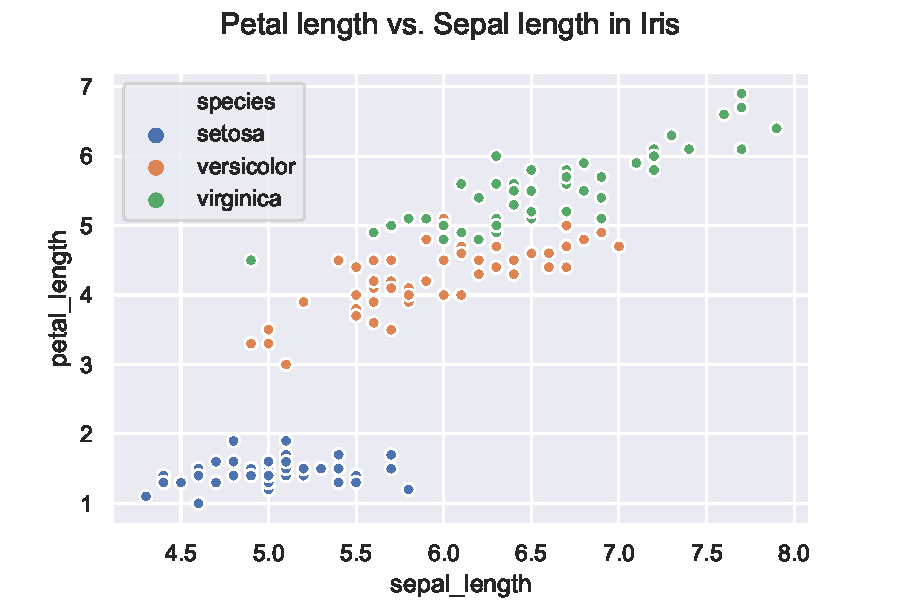
\includegraphics[width=0.7\textwidth]{scatter.pdf}
    \end{center}
    

\end{frame}

\begin{frame}{Generalizando}{Discreto y aproximable}

    \dots generalizamos.

    \begin{center}
        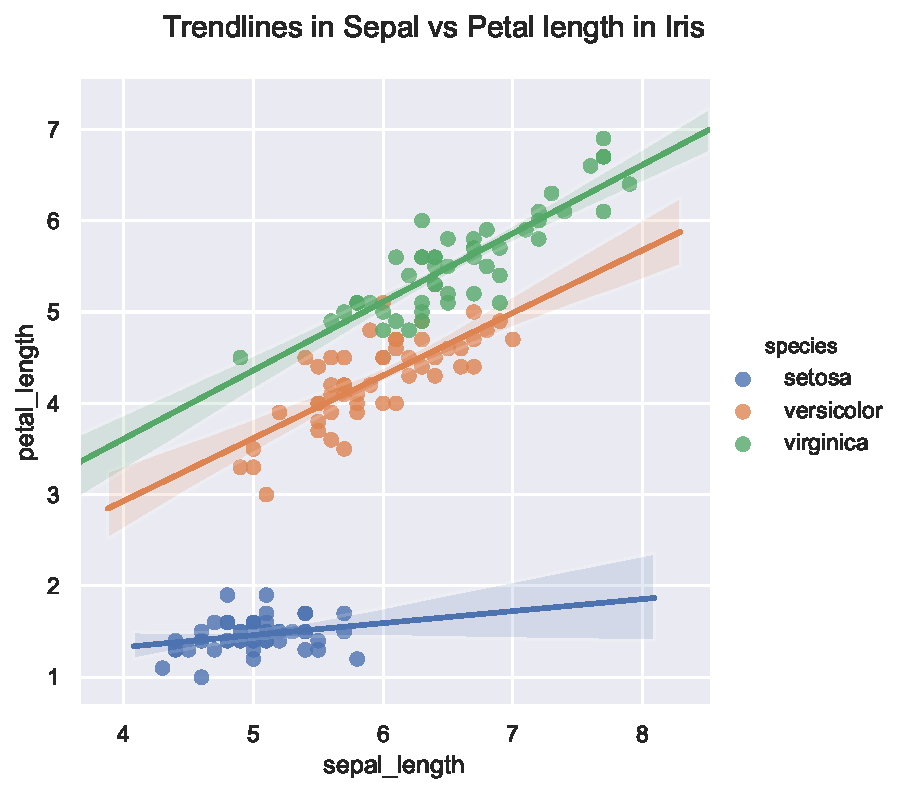
\includegraphics[width=0.62\textwidth]{regplot.pdf}
    \end{center}
    

\end{frame}

% Específicamente, la regla 3 puede verse como $R_i = R_i - \frac{a_{ik}}{a_{jk}}R_j$.

% Los robots
% why is it important
% does it exist in math?
% how to represent it
% how to represent it in matlab
% practical cases

% \section*{Referencias}

% \begin{frame}[t]{Referencias}
    % \nocite{bibID01}
    % \nocite{bibID02}

    % \bibliographystyle{IEEE}
    % \bibliography{biblio}
% \end{frame}

\end{document}